\documentclass[tikz,border=0pt]{standalone}
\usepackage{xcolor}
\usepackage{tikz}
\usetikzlibrary{calc,angles,quotes}
\usetikzlibrary{intersections}
\usepackage{amsmath}
\usepackage{lmodern}
\usepackage[latin2]{inputenc}

\begin{document}
\begin{tikzpicture}

\node (a) at (0,0){
\includegraphics[scale=1]{Figure3_pre.pdf}
};

\node (b) at (-0,6.75){
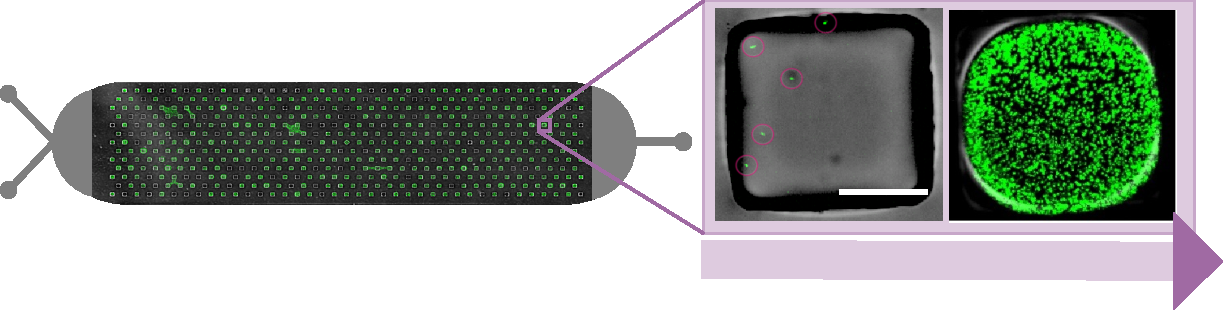
\includegraphics[scale=0.725]{chip.pdf}
};

\node at (-7.5,8.5)[font=\fontsize{11}{11} \selectfont]{(a)};


\node at (-6.75,7.8)[font=\fontsize{11}{11} \selectfont]{inlets};
\node at (-3,5.45)[font=\fontsize{11}{11} \selectfont]{500 droplets: 2 nl/droplets};
\node at (0.5,7.8)[font=\fontsize{11}{11} \selectfont]{outlet};

\node at (3.3,6.55)[font=\fontsize{11}{11} \selectfont,color=white]{$60 \mu m$};

\node at (2.75,5.45)[font=\fontsize{11}{11}\selectfont]{day 1};
\node at  (5.5,5.45)[font=\fontsize{11}{11} \selectfont]{day 2};


\end{tikzpicture}
\end{document}